\begin{figure}[H]
    \centering
    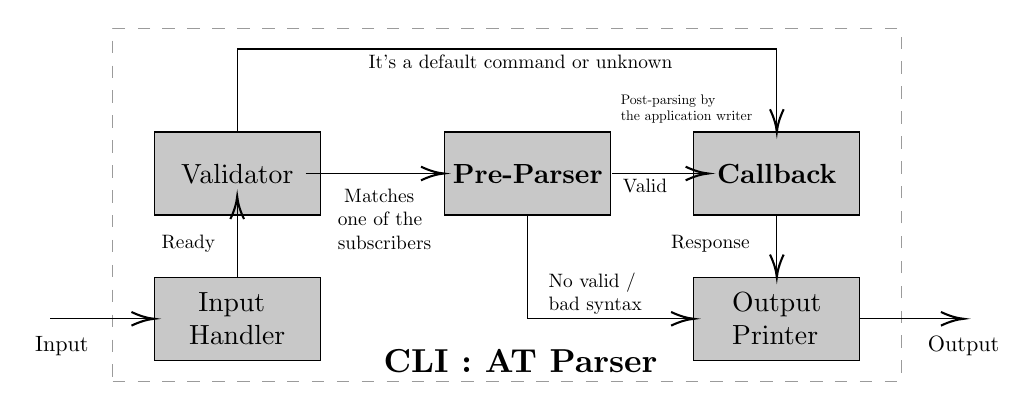
\begin{tikzpicture}[x=0.75pt,y=0.75pt,scale=1]
        \draw  [color={rgb, 255:red, 155; green, 155; blue, 155 }  ,draw opacity=1 ][fill={rgb, 255:red, 255; green, 255; blue, 255 }  ,fill opacity=1 ][dash pattern={on 4.5pt off 4.5pt}] (80,70) -- (460,70) -- (460,240) -- (80,240) -- cycle ;
        \draw  [fill={rgb, 255:red, 200; green, 200; blue, 200 }  ,fill opacity=1 ] (100,80) -- (180,80) -- (180,120) -- (100,120) -- cycle ;
        \draw  [fill={rgb, 255:red, 200; green, 200; blue, 200 }  ,fill opacity=1 ] (100,150) -- (180,150) -- (180,190) -- (100,190) -- cycle ;
        \draw  [fill={rgb, 255:red, 200; green, 200; blue, 200 }  ,fill opacity=1 ] (240,150) -- (320,150) -- (320,190) -- (240,190) -- cycle ;
        \draw  [fill={rgb, 255:red, 200; green, 200; blue, 200 }  ,fill opacity=1 ] (360,150) -- (440,150) -- (440,190) -- (360,190) -- cycle ;
        \draw  [fill={rgb, 255:red, 200; green, 200; blue, 200 }  ,fill opacity=1 ] (360,80) -- (440,80) -- (440,120) -- (360,120) -- cycle ;
        \draw    (140,190) -- (140,230) -- (400,230) -- (400,192) ;
        \draw [shift={(400,190)}, rotate = 450] [color={rgb, 255:red, 0; green, 0; blue, 0 }  ][line width=0.75]    (10.93,-3.29) .. controls (6.95,-1.4) and (3.31,-0.3) .. (0,0) .. controls (3.31,0.3) and (6.95,1.4) .. (10.93,3.29)   ;
        \draw    (50,100) -- (98,100) ;
        \draw [shift={(100,100)}, rotate = 180] [color={rgb, 255:red, 0; green, 0; blue, 0 }  ][line width=0.75]    (10.93,-3.29) .. controls (6.95,-1.4) and (3.31,-0.3) .. (0,0) .. controls (3.31,0.3) and (6.95,1.4) .. (10.93,3.29)   ;
        \draw    (440,100) -- (488,100) ;
        \draw [shift={(490,100)}, rotate = 180] [color={rgb, 255:red, 0; green, 0; blue, 0 }  ][line width=0.75]    (10.93,-3.29) .. controls (6.95,-1.4) and (3.31,-0.3) .. (0,0) .. controls (3.31,0.3) and (6.95,1.4) .. (10.93,3.29)   ;
        \draw    (400,150) -- (400,122) ;
        \draw [shift={(400,120)}, rotate = 450] [color={rgb, 255:red, 0; green, 0; blue, 0 }  ][line width=0.75]    (10.93,-3.29) .. controls (6.95,-1.4) and (3.31,-0.3) .. (0,0) .. controls (3.31,0.3) and (6.95,1.4) .. (10.93,3.29)   ;
        \draw    (280,150) -- (280,100) -- (358,100) ;
        \draw [shift={(360,100)}, rotate = 180] [color={rgb, 255:red, 0; green, 0; blue, 0 }  ][line width=0.75]    (10.93,-3.29) .. controls (6.95,-1.4) and (3.31,-0.3) .. (0,0) .. controls (3.31,0.3) and (6.95,1.4) .. (10.93,3.29)   ;
        \draw (400,170) node  [align=left] {\textbf{Callback}};
        \draw (280,170) node  [align=left] {\textbf{Pre-Parser}};
        \draw (140,170) node  [align=left] {Validator};
        \draw (400,100) node  [align=left] {Output\\Printer};
        \draw (140,100) node  [align=left] { \ Input\\Handler};
        \draw (55.5,87) node [scale=0.8] [align=left] {Input};
        \draw (490,87) node [scale=0.8] [align=left] {Output};
        \draw (368,136) node [scale=0.7] [align=left] {Response};
        \draw (336.5,164) node [scale=0.7] [align=left] {Valid};
        \draw (211,148) node [scale=0.7] [align=left] { \ Matches\\ one of the\\subscribers};
        \draw (276.5,224) node [scale=0.7] [align=left] {It's a default command or unknown};
        \draw (312.5,112) node [scale=0.7] [align=left] {No valid /\\bad syntax};
        \draw (356.5,201) node [scale=0.5] [align=left] {Post-parsing by \\the application writer};
        \draw (116.5,136) node [scale=0.7] [align=left] {Ready};
        \draw (276.5,79.5) node [scale=1.2] [align=left] {\textbf{CLI : AT Parser}};
        \draw    (173,170) -- (237.5,170) ;
        \draw [shift={(239.5,170)}, rotate = 180] [color={rgb, 255:red, 0; green, 0; blue, 0 }  ][line width=0.75]    (10.93,-3.29) .. controls (6.95,-1.4) and (3.31,-0.3) .. (0,0) .. controls (3.31,0.3) and (6.95,1.4) .. (10.93,3.29)   ;
        \draw    (320.5,170) -- (365,170) ;
        \draw [shift={(367,170)}, rotate = 180] [color={rgb, 255:red, 0; green, 0; blue, 0 }  ][line width=0.75]    (10.93,-3.29) .. controls (6.95,-1.4) and (3.31,-0.3) .. (0,0) .. controls (3.31,0.3) and (6.95,1.4) .. (10.93,3.29)   ;
        \draw    (140,120) -- (140,157) ;
        \draw [shift={(140,159)}, rotate = 270] [color={rgb, 255:red, 0; green, 0; blue, 0 }  ][line width=0.75]    (10.93,-3.29) .. controls (6.95,-1.4) and (3.31,-0.3) .. (0,0) .. controls (3.31,0.3) and (6.95,1.4) .. (10.93,3.29)   ;
    \end{tikzpicture}
    \caption{AT parser for a CLI implementation}
    \label{fig:atparser}
\end{figure}